\chapter{Characterization}

Our work focuses on characterizing the energy and latency of end-to-end Omni-directional-stereo(ODS) Camera  system. The goal is to find the bottlenecks of different components in the hardware and software pipeline and propose optimizations. As the existing ODS camera systems are built from off the shelf camera devices and the conventional stitching algorithms we see a potential research opportunity to close gaps between hardware and software. Many existing systems like Google Jump, Facebook Surround capture and compute on enormous amount of data consuming several hundreds of watts of total energy to stitch ODS in realtime 30fps. The main challenge in ODS generation is to understand the data flow across the system and to make decisions on data abstractions needed at different subcomponents to reduce the total system power.

Many have argued [Edvardo Hotmobile, Nvidia, AMD] that we need resolutions greater than 16k and frame-rate greater of 240 for true immersion in VR. At such higher framerate and resolutions there is lot of information that is redundantly captured, processed and transferred. Therefore, in our work, we study how the energy and latency of each stage get affected by the output resolution and the characterize the bottlenecks in greater detail. 

We characterize both monoscopic and ODS camera systems. The difference between them is the number of novel views needed is significantly higher for ODS. Monoscopic is a special case of ODS and at core involves the same optical flow based stitching. So we will characterize generalized flow based stitching system and notify any important differences between monoscopic and ODS when necessary.\newline

\section{Energy Measurement Methodology}

The end to end camera system, as shown in figure 3.1 can be divided into 4 major stages by energy consumption, viz., image sensor, image signal processor(ISP), processing, and Off-chip memory. For our prototype design ODS design we use six imx-274 cameras for capture and Nvidia Jetson TX2 for processing the frames. The Camera and Jetson specs are shown in figure 3.2. Jetson has power moniter IC and ways to moniter CPU, GPU, memory frequencies. We compute the energy of each individual stage by measuring the difference between the idle and active stage(when capturing/computing).
(
Prototype System Overview \newline
Hardware:
System 1) Dual Fisheye Camera for monoscopic 360
System 2) Six Camera Rig for OmniDrirectional Stereo
)
Jetson power monitering , IO Power
Micron System Power Calculator for LPDDR2. \newline

Software:
Camera API,
openCV, C++
\newline

1) Energy/Power \newline
	a) Individual Stage Power Characterization. 
	%figure
	X axis has different stages and Y axis correspond to energy per frame \newline
	\begin{tabular}{c|c|c|c}
		Stage & Substage & Data Type/Domain/Format & Typical Size \\
		\multirow{3}{*}{ Camera } & CIS & Analog Voltage/Current & Pixel \\
		& ADC & Quantized Bits & Pixel Depth \\
		& IO & Bayer/ Raster output & Row/Coloumn of Pixels \\
		\multirow{4}{*}{ ISP } & Raw Processing & Bayer & Set of lines \\
		& Demosaic & Bayer to RGB & Set of lines \\
		& Color Correction & RGB & Set of lines \\
		& Codec & RGB & Frame / Set of Frames \\
		\multirow{5}{*}{ Computation } & Distortion Corr. & RGB & Full Frame \\
		& Projection & RGB & Full Frame \\
		& Optical Flow & Gray & Two Adjacent Frames, Pyramids \\
		& View Synthesis & RGB & OF + Frames \\
		& Sharpening & RGB & Frame \\
	\end{tabular} 
\newline

	b) Breakdown of Individual Stage
		Camera Sensor and ISP power directly taken from literature.
		Computation Power split into sub stages. \newline
		For power characterization of camera sensor and ISP, we run the camera in different resolutions and framerates and see how the various sub-component power changes. The components include Camera Sensor, I/O, ISP, CODEC, DDR, and CPU. The ISP, and CODEC power are combined as they belong to same SOC voltage rail.
		
		The most used configuration for our project when all the six cameras are capturing 1920x1080 @ 30 fps. At this configuration below is the split of different component power. \newline
		
		\begin{tabular}{c|c|c|c}
			Power Rail  & Diff. Current(mA) & Voltage(mV) & Power(mW)   \\
			$ISP+CODEC$ & 102.7             & 19152       & 1966.9      \\
			$CPU$ & 16.4              & 19144       & 314.0       \\
			$DDR$ & 260.4             & 4792        & 1247.8      \\
			$CAM\_SNSR$ & 375.4             & 3336        & 1252.3      \\
			Total       & -                 & -           & 4781.0      \\
		\end{tabular} \newline
		
		Although we built a system where all the cameras are capturing at same resolution and framerate at a given time, we expect the future cameras make these decisions dynamically to save power. Therefore, we  measure the efficiency of capture and ISP processing at different modes of operation and measure the efficiency of capture and processing in power consumed per pixel at different modes.
		
% Figure 
\begin{figure*}
	\begin{center}
		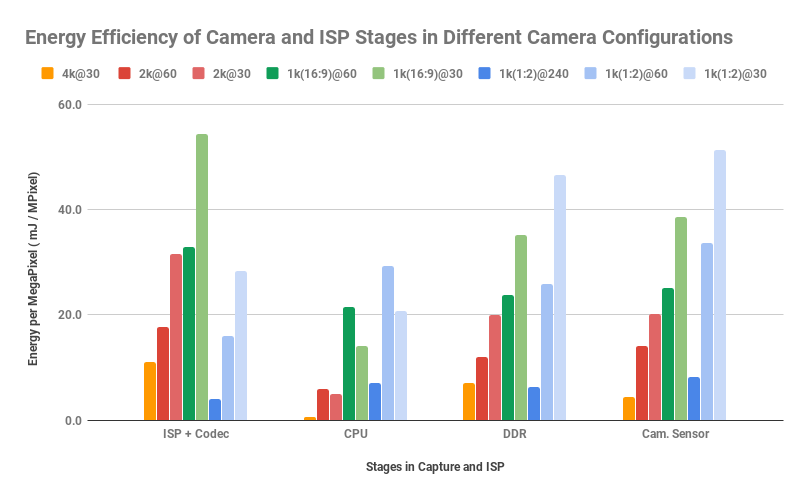
\includegraphics[width=1\textwidth]{/media/gunman/Data/thesis/ThesisLatex/data/images/Power_Efficiency_of_Camera_ISP_Stages_in_different_configurations.png}
		\caption{Power Efficiency of Camera ISP Stages in different configurations}
		\label{fig:ex_4_9}
	\end{center}
	\vspace{-0.3in}
\end{figure*} 


d) Scaling with the resolution\newline
Outputs:
4k, 6k, 8k, 12k
Discuss scalability of resolution for different stages. \newline
Especially the scalability of cache, DRAM, CPU power. 
\begin{figure*}
	\begin{center}
		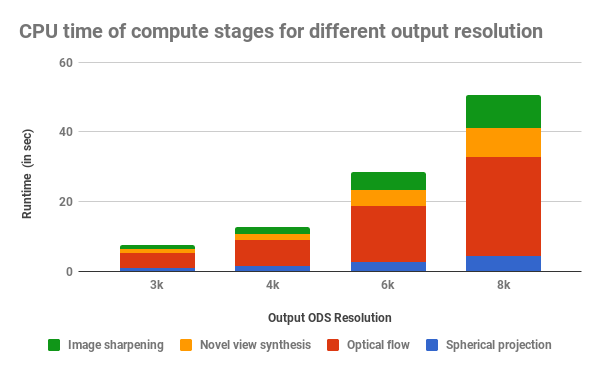
\includegraphics[width=1\textwidth]{/media/gunman/Data/thesis/ThesisLatex/data/images/ExecutionTimeComputeStages.png}
		\caption{CPU execution time of different compute stages}
		\label{fig:ex_4_9}
	\end{center}
	\vspace{-0.3in}
\end{figure*} 

What is the energy per each output pixel	
What is energy per pixel when generating only one ODS view, and how does it compare when generating two views! If it is double then we have a pproblem to solve	
Check why sharpening is so costly!	

d) Increased frame-rate\newline
		What is the percentage of new data
			ffmpeg I-frame size to the P-frame ratio.
			\begin{figure*}
				\begin{center}
					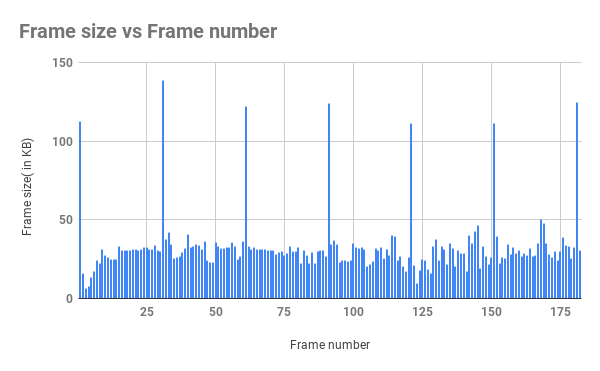
\includegraphics[width=1\textwidth]{/media/gunman/Data/thesis/ThesisLatex/data/images/FramesizevsFramenumber.png}
					\caption{Framesize of I and P frames}
					\label{fig:ex_4_9}
				\end{center}
				\vspace{-0.3in}
			\end{figure*} 
		%ffprobe lab.mp4 -show_frames
		we usually have I,P, and B frames in a compressed video, but in case of realtime compression we will have only I and P frames and disable B frames as it adds latency to the pipeline. Typically I-frame to P-frame is about ~4 times and one I-frame occur for ~30 P-frames. This implies we save a lot on interface power if we can push the computation to near sensor.  
		[Numbers - savings from IO datarate reduction]
			
	e) Quality Tradeoff's with input resolution\newline
			Sharpening
			Reducing number of pyramid's
	f) High motion Vs low motion differences
	g) File IO power
	h) Breakdown in terms of type of Memory	used
	i) Breakdown in terns of type of Computation
	j) Breakdown in terms of IO bandwidth bottlenecks
	
	

2) Performance \newline
	a) Individual Stage Latency Characterization
	b) Breakdown of Optical Flow
		Individual Stage
		Time for each Pyramid Generation
	c) Breakdown of sharpening
	

